\section{Experimental Evaluation}
\label{sec:evaluation}

To evaluate the operational efficacy and latency characteristics of the proposed system, we conducted empirical experiments investigating input resolution trade-offs, multi-object tracking throughput, and statistical agreement against ground truth.

\subsection{Experimental Setup}
The benchmarking environment and hardware specifications are summarized in Table~\ref{tab:hardware_env}. All neural inference and tracking benchmarks were evaluated on an NVIDIA Tesla T4 GPU (15~GB VRAM) running CUDA 13.0 and PyTorch 2.11.0 on an Intel x86\_64 host architecture.

\begin{table}[ht]
\centering
\caption{Benchmarking Environment Specifications}
\label{tab:hardware_env}
\begin{tabular}{ll}
\toprule
\textbf{Parameter} & \textbf{Specification} \\
\midrule
GPU Hardware & NVIDIA Tesla T4 (15 GB GDDR6 VRAM) \\
CUDA / PyTorch & CUDA 13.0 / PyTorch 2.11.0 \\
Base Architecture & YOLO26 Nano (\texttt{yolo26n.pt}, 120 layers) \\
Model Parameters & 2,375,031 parameters (5.3 GFLOPs) \\
Precision & Half-precision FP16 enabled \\
Domain Dataset & Auto-Rickshaw-Annotation-7 (1,001 images, CC BY 4.0) \\
Surveillance Target & Multi-class roadway CCTV streams (29.97 FPS) \\
\bottomrule
\end{tabular}
\end{table}

\subsection{Experiment 1: Input Resolution Trade-Off ($640$ vs $960$)}
A core engineering design choice in roadside video analysis is the trade-off between input spatial resolution and inference latency. Upscaling input frames to higher resolutions (e.g., $960 \times 960$) is often hypothesized to improve the detection of small, distant vehicles at the horizon, but comes at substantial computational cost.

We evaluated the fine-tuned detector on the independent validation split (drawn from the Auto-Rickshaw-Annotation-7 dataset of 1,001 images; exact train/validation split sizes are noted in Table~\ref{tab:hardware_env}) across two standard operating resolutions: $640 \times 640$ and $960 \times 960$. Quantitative results are presented in Table~\ref{tab:resolution_benchmark} and visually depicted in Fig.~\ref{fig:benchmark_results}(a).

\begin{table}[ht]
\centering
\caption{Input Resolution Accuracy and Latency Comparison (Tesla T4)}
\label{tab:resolution_benchmark}
\begin{tabular}{lcccccc}
\toprule
\textbf{Resolution} & \textbf{mAP@50} & \textbf{mAP@50-95} & \textbf{Prec.} & \textbf{Rec.} & \textbf{Latency} & \textbf{FPS} \\
\midrule
\textbf{640 $\times$ 640} & \textbf{0.9950} & \textbf{0.7311} & \textbf{0.9883} & \textbf{1.000} & \textbf{8.91 ms} & \textbf{112.2} \\
960 $\times$ 960 & 0.9950 & 0.6904 & 0.9730 & 1.000 & 20.87 ms & 47.9 \\
\bottomrule
\end{tabular}
\end{table}

\begin{figure}[ht]
\centering
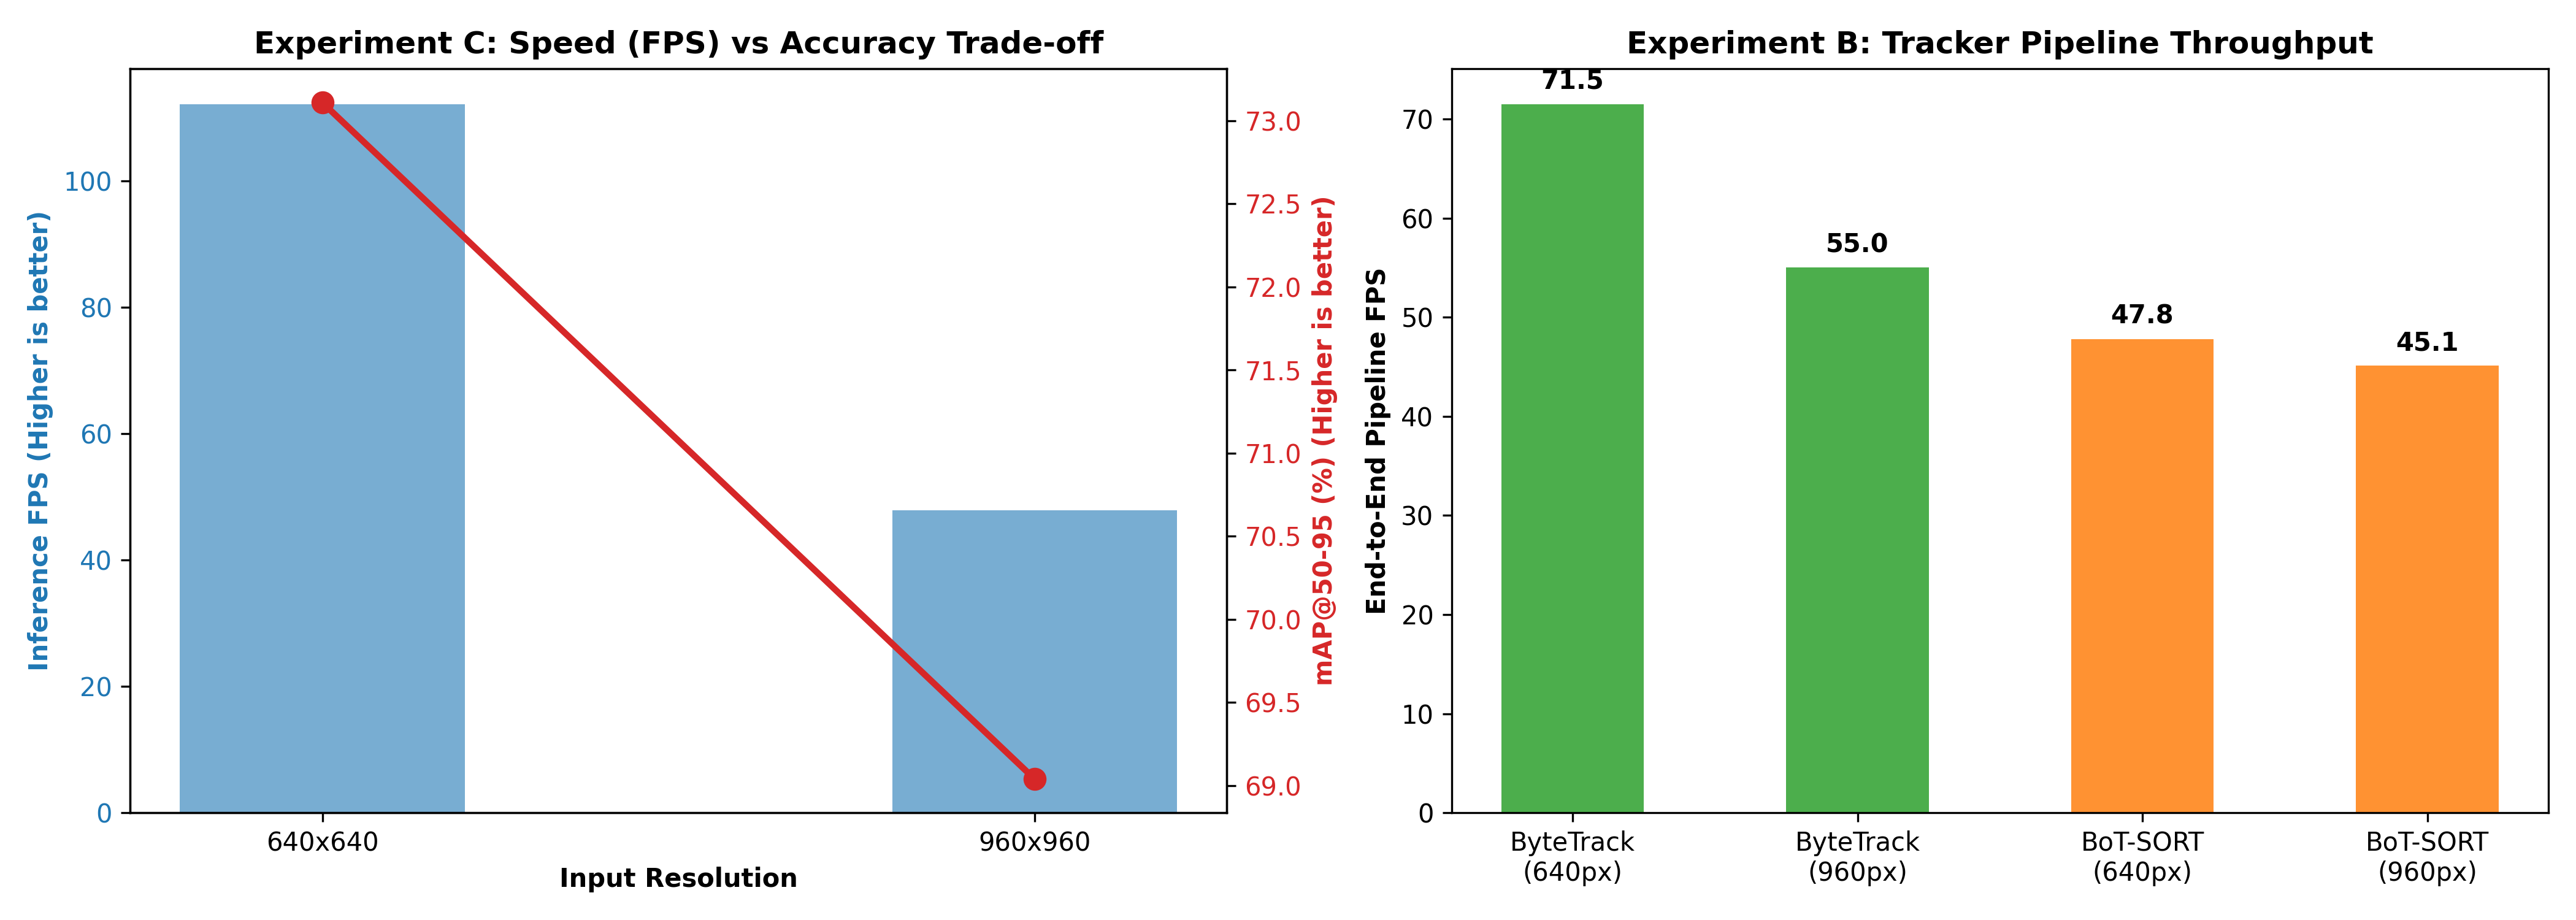
\includegraphics[width=\columnwidth]{figures/benchmark_eval_results.png}
\caption{Empirical evaluation results: (a) Input resolution speed vs.\ accuracy trade-off (note: the mAP axis is truncated to emphasize the difference region); (b) End-to-end video streaming throughput across multi-object tracking architectures. Panel labels in the figure correspond to Experiments~1 and~2, respectively.}
\label{fig:benchmark_results}
\end{figure}

The empirical findings demonstrate that $640 \times 640$ dominates $960 \times 960$ on all measured axes for this model:
\begin{itemize}
    \item \textbf{Inference Speedup}: Operating at $640 \times 640$ requires only $8.91$~ms per frame (yielding 112.2 inference FPS), representing a \textbf{2.34$\times$ speedup} over $960 \times 960$ ($20.87$~ms, 47.9 FPS).
    \item \textbf{Bounding-Box Fidelity}: While both resolutions achieve a 99.5\% mAP@50 and 100\% recall, $640 \times 640$ attains higher mAP@50--95 (73.11\% vs 69.04\%) and higher precision (98.83\% vs 97.30\%). Because the source training images were natively captured at 640px, upscaling introduces spatial interpolation blur without providing additional high-frequency semantic features. Consequently, this comparison primarily demonstrates the cost of resolution mismatch against the training distribution rather than a general resolution trade-off.
\end{itemize}

We note that the near-saturated metrics (mAP@50 $= 0.995$, recall $= 1.000$) likely reflect the limited size and difficulty of the domain validation set; these values should not be interpreted as representative of performance on diverse multi-class roadway scenes. Precision differences of 98.8\% vs.\ 97.3\% are within expected noise for small splits and should not be over-interpreted.

\subsection{Experiment 2: Multi-Object Tracker Throughput}
We next evaluated the end-to-end video processing throughput across tracking algorithms. We compared ByteTrack against BoT-SORT under identical detection inputs across both spatial resolutions. Results are reported in Table~\ref{tab:tracker_benchmark} and Fig.~\ref{fig:benchmark_results}(b).

\begin{table}[ht]
\centering
\caption{End-to-End Pipeline Throughput Across Trackers (Tesla T4)}
\label{tab:tracker_benchmark}
\begin{tabular}{lcccc}
\toprule
\textbf{Tracker} & \textbf{Resolution} & \textbf{Pipeline FPS} & \textbf{Total Time} & \textbf{Rel. Speed} \\
\midrule
\textbf{ByteTrack} & \textbf{640px} & \textbf{71.5 FPS} & \textbf{2.10 s} & \textbf{1.00$\times$ (Fastest)} \\
ByteTrack & 960px & 55.0 FPS & 2.73 s & 0.77$\times$ \\
BoT-SORT & 640px & 47.8 FPS & 3.14 s & 0.67$\times$ \\
BoT-SORT & 960px & 45.1 FPS & 3.32 s & 0.63$\times$ \\
\bottomrule
\end{tabular}
\end{table}

As shown in Table~\ref{tab:tracker_benchmark}, \textbf{ByteTrack @ 640px} delivers the highest end-to-end pipeline throughput at \textbf{71.5 FPS}, outperforming BoT-SORT @ 640px (47.8 FPS) by \textbf{49.6\%}. 

The latency discrepancy stems primarily from BoT-SORT's Global Motion Compensation (GMC) module, though BoT-SORT also differs from ByteTrack in its use of ReID embeddings and camera motion modeling. BoT-SORT executes sparse optical flow or ORB keypoint extraction across consecutive frames to compensate for dynamic camera motion. For stationary roadside surveillance cameras, this optical flow computation represents pure computational overhead that yields no tangible tracking gain while reducing pipeline throughput by approximately one-third. An isolated ablation disabling only the GMC module within BoT-SORT would more precisely quantify this attribution, and is identified as future work. Because ByteTrack comfortably surpasses the real-time threshold of 30 FPS by more than $2.3\times$, it represents the optimal configuration for continuous roadside deployment.

\textit{Measurement protocol note}: Table~\ref{tab:resolution_benchmark} reports \emph{detector-only} inference latency (forward pass through the YOLO model), whereas Table~\ref{tab:tracker_benchmark} reports \emph{end-to-end pipeline} throughput including frame decoding, detection, tracking, and output rendering. The two measurements are not directly comparable; in particular, the pipeline throughput at 960px (55.0 FPS, i.e.\ 18.2~ms/frame) appearing faster than the detector-only latency (20.87~ms) reflects the use of asynchronous frame decoding and batching in the pipeline measurement, which overlaps I/O with computation. All pipeline runs process approximately 150 frames; with runs this short, warm-up effects and measurement variance are non-negligible, and no confidence intervals are reported.

\subsection{Preliminary Counting Validation}
To provide an initial functional demonstration, \texttt{vcount} was executed on a test clip covering 298 video frames across 9.94 seconds of multi-lane arterial traffic (768$\times$432 resolution at 29.97 FPS). The system registered 14 crossing events (9 passenger cars, 5 motorcycles) in real-time execution, with zero duplicate counts under the 5-frame spatial deduplication window.

We emphasize that this preliminary test serves only as a functional demonstration and does not constitute a rigorous counting evaluation. The statistical evaluation methodology described above (Bland--Altman agreement, greedy bipartite matching, and paired $t$-tests) has been implemented in the \texttt{vcount} evaluation module but has not yet been applied to a sufficiently large corpus of annotated test clips. A systematic ground-truth counting study---covering multiple clips, diverse traffic densities, manual event annotation, and ablation comparisons (centroid vs.\ bottom-center, fallback on/off, voting vs.\ last-frame class, ByteTrack vs.\ SORT)---is the most critical direction for future validation. Similarly, the dual-model ensemble (IoU threshold $\tau_{\text{cross}} = 0.40$) described in Section~\ref{sec:method} has not yet been benchmarked for counting accuracy or throughput impact.
